\section{System Architecture}
\label{sec:architecture}

This section presents the overall architecture of the Slurm Agent system, describing the major components, their interactions, and the rationale behind architectural decisions. The architecture follows a layered design that separates user interface, agent logic, and system integration concerns.

\subsection{Architecture Overview}

The Slurm Agent system consists of four main layers:

\begin{enumerate}
    \item \textbf{Presentation Layer}: Web-based frontend for user interaction
    \item \textbf{Agent Layer}: Multi-agent backend handling reasoning and orchestration
    \item \textbf{Protocol Layer}: MCP server providing standardized tool interfaces
    \item \textbf{Infrastructure Layer}: Slurm cluster and external services
\end{enumerate}

% Placeholder: System architecture diagram
\begin{figure}[H]
    \centering
    % \fbox{\parbox{0.8\textwidth}{\centering \textit{[Placeholder: Complete system architecture diagram showing all layers and component interactions]}}}
    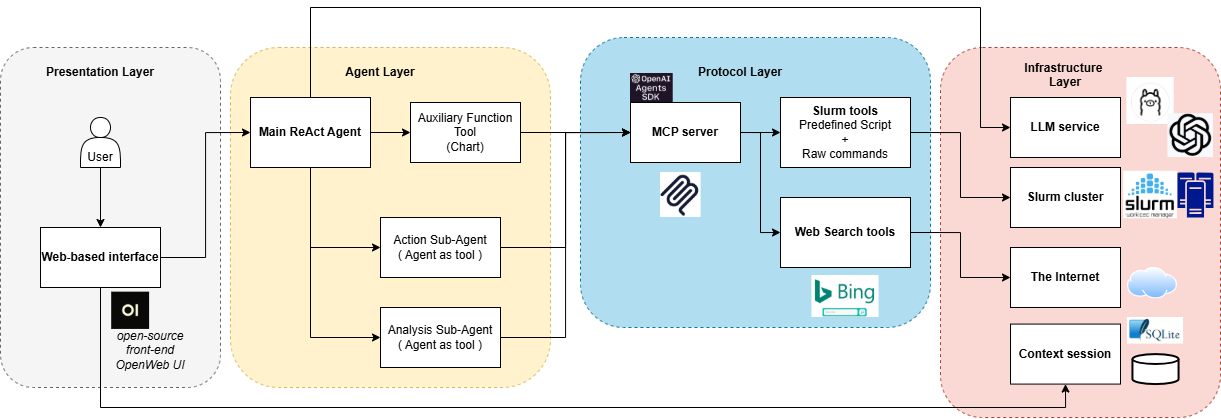
\includegraphics[width=1\textwidth]{images/agent_system_architect.drawio.png}
    \caption{Slurm Agent System Architecture}
    \label{fig:system-architecture}
\end{figure}

\subsection{Component Descriptions}

\subsubsection{Presentation Layer}

The Presentation Layer provides the user-facing interface for interacting with the Slurm Agent. This layer is responsible for:

\begin{itemize}
    \item Rendering a conversational chat interface with message history
    \item Capturing user queries in natural language
    \item Displaying streaming responses in real-time
    \item Rendering formatted content including markdown, code blocks, and inline visualizations
    \item Managing confirmation workflows for dangerous operations
    \item Preserving session state across interactions
\end{itemize}

The interface follows a conversational paradigm where users type queries and receive responses in a familiar messaging format. This design abstracts the complexity of Slurm commands behind natural language interaction.

\subsubsection{Agent Layer}

The Agent Layer implements the core reasoning and orchestration logic using a multi-agent architecture. The system employs a hierarchical structure with specialized agents:

\begin{itemize}
    \item \textbf{Main ReAct Agent}: The primary orchestrator that implements the Think $\rightarrow$ Act $\rightarrow$ Observe reasoning loop. This agent maintains conversation context, interprets user intent, and delegates to specialized sub-agents based on the nature of the request.
    
    \item \textbf{Analysis Sub-Agent}: Handles read-only information gathering operations including cluster status queries, job queue inspection, resource monitoring, and documentation search. This agent can chain multiple tool calls to gather comprehensive information.
    
    \item \textbf{Action Sub-Agent}: Manages operations that modify cluster state, such as job submission, cancellation, and configuration changes. This agent enforces safety controls and confirmation requirements for dangerous operations.
\end{itemize}

The Main Agent also has direct access to auxiliary tools including chart generation for data visualization, which calls the Protocol Layer to render cluster metrics and statistics as visual charts.

Key architectural features of the Agent Layer include:
\begin{itemize}
    \item \textbf{Session Persistence}: Conversation history is maintained across interactions, enabling contextual follow-up queries
    \item \textbf{Confirmation Workflow}: Dangerous operations are queued pending explicit user confirmation before execution
    \item \textbf{Token Optimization}: Visualization artifacts are filtered from conversation history to reduce token consumption
    \item \textbf{Streaming Output}: Responses are streamed incrementally to provide immediate user feedback
\end{itemize}

\subsubsection{Protocol Layer}

The Protocol Layer implements the Model Context Protocol (MCP) to provide a standardized interface between the Agent Layer and the underlying Slurm infrastructure. This layer:

\begin{itemize}
    \item \textbf{Exposes Slurm Operations as Tools}: Each Slurm command is wrapped as a discrete tool with defined parameters and return types
    \item \textbf{Validates Parameters}: Input validation prevents malformed or dangerous command construction
    \item \textbf{Executes Commands Safely}: Commands are executed with appropriate isolation and error handling
    \item \textbf{Formats Output}: Raw command output is processed into structured formats suitable for agent consumption
\end{itemize}

The MCP abstraction provides several benefits:
\begin{itemize}
    \item Decouples agent logic from Slurm-specific implementation details
    \item Enables tool discovery and introspection by the agent
    \item Supports extension with new tools without modifying the agent core
    \item Provides a security boundary for command execution
\end{itemize}

\subsubsection{Infrastructure Layer}

The Infrastructure Layer comprises the external systems that the agent interacts with:

\begin{itemize}
    \item \textbf{Large Language Model}: Provides the reasoning capabilities for natural language understanding, intent interpretation, and response generation (either local or cloud API)
    \item \textbf{Slurm Cluster}: The target HPC infrastructure being managed, accessed through standard Slurm commands
    \item \textbf{Web Search Service}: Enables retrieval of documentation and troubleshooting information from external sources
    \item \textbf{Context Database}: SQLite database for storing session state and pending confirmation actions
\end{itemize}

\subsection{Communication Patterns}

The architecture employs several communication patterns:

\textbf{Request-Response}: Standard requests for initiating conversations and submitting queries.

\textbf{Streaming}: Unidirectional streaming from backend to frontend for real-time response delivery. The backend sends a continuous stream of events that the frontend processes incrementally.

\textbf{Tool Invocation}: Structured communication between the Agent Layer and Protocol Layer for tool discovery and execution.


\subsection{Data Flow}

A typical query flows through the system layers as follows:
\begin{enumerate}
    \item User submits natural language query through the Presentation Layer
    \item Agent Layer receives query and begins Think-Act-Observe reasoning
    \item Agent delegates to appropriate sub-agent based on query type
    \item Sub-agent invokes tools via Protocol Layer to gather data or perform actions
    \item Results propagate back through the layers
    \item Agent synthesizes response and streams to user
\end{enumerate}

For dangerous operations, an additional confirmation step interrupts the flow: the pending action is stored and presented to the user, and execution proceeds only after explicit confirmation.

\subsection{Deployment Architecture}

The system components can be deployed in various configurations:

\textbf{Local Development}: All components run on a single machine with local Slurm installation or connection to a remote cluster.

\textbf{Distributed Deployment}: Frontend, backend, and MCP server run on separate hosts, with the MCP server deployed on a Slurm management node.

The modular architecture supports flexible deployment topologies based on infrastructure requirements and security considerations.
